\documentclass[addpoints,12pt]{exam}

\usepackage{amsmath}
\usepackage{amsthm}
\usepackage{graphicx}
\usepackage{enumitem}
\usepackage{comment}

\newtheorem{theorem}{Theorem}

\printanswers %Remove to hide answers
\pagestyle{headandfoot} %Adds Headers and Footers
\runningheadrule
\firstpageheader{Math 151}{Exam 1}{\today}
\runningheader{Math 151}
{Exam 1, Page \thepage\ of \numpages}
{\today}
\firstpagefooter{}{\thepage}{}
\runningfooter{}{\thepage}{}


\begin{document}

%The box at the top, and the name
\begin{center}
\fbox{\fbox{\parbox{5.5in}{\centering
You are allowed a calculator on this exam. All other notes and help are not allowed. Scratch paper will be provided upon request. All work on scratch paper will not be graded. \textbf{To recieve full credit, you must show your work. 
} Feel free to leave answers unsimplified. Best of luck, I am rooting for you. 
}}}
\end{center}
\vspace{0.1in}
\makebox[\textwidth]{Name:\enspace\hrulefill}
\vspace{0.2in}

%Question Formatting
%\qformat{\textbf{Question \thequestion}\quad (\thepoints)\hfill}
%Point Table


%\begin{center}
%\gradetable[h][questions]
%\end{center}

%Beginning Questions
\begin{questions}
	\question Solve the following linear equation. 
   \[
 x-2 = -3(x-2)+8~.
\]\vfill

\begin{comment}
\question Solve the following equation 
\[
 \frac{x}{5}- \frac{1}{2} = \frac{x}{6}~.
\]

\end{comment}


\question The length of an American football field is 200 feet more than its width. If the perimeter is 1040 feet, then how wide is the field? \vfill


\begin{comment}
\question You have 150 dollars to invest. Part of the money is invested in an account through Yankton Financial paying $15\%$ annual interest. The rest of the money is to be invested in a second account at Vermillian Bank paying $13\%$ interest. If you would like $\$20$ a year in interest, how much should you invest into each account? Feel free to keep your answer unsimplified. 
\end{comment}

\begin{comment}
\question Perform the following computation using complex numbers. 
   \[
		 (7+2i)-(5-7i)= 
\]
\end{comment}



\question Perform the following computation using complex numbers. 
\[
		 (2+i)(-3-i)=
\] \vfill

\newpage

\question Solve the following quadratic equation by factoring~. 
\[
	x^{2}-x-6=0 
\]

\vfill


\begin{comment}
\question Solve the following quadratic equation by the square root property. 
   \[
   5x^{2}+1=26
   \]
\end{comment}

\question Solve the following quadratic equation by using the quadratic formula. (Formula on Last Page)
   \[
x^{2}+2x-4=0
\]

\vfill

\begin{comment}
\question Solve the following equation involving radicals~.
   \[
    \sqrt{2x-1}=x
	 \]
\end{comment}

\question  Solve the following equation involving an absolute value. 
	    \[
	  |x-2|-2=1
	 \]
\vfill
\newpage

\question Give each interval using interval notation.
\begin{enumerate}[label = \alph*)]
    \item $ 4 < x \leq 5 $  \vspace{20pt} 
		\item $ x\geq  -2 $ \vspace{20pt} 
		\item $-2 \leq x \leq  5 $ \vspace{20pt} 
		\item $x \leq 3 $  \vspace{20pt} 
\end{enumerate}

\question Solve the following linear inequality. 
   \[
-4(x+1)+2\geq 3x-9
\]
\vfill
\begin{comment}
\question Solve the absolute value inequality 
\[
|3x-9| > 3
\]
\end{comment}

\question Solve the following system of linear equations. 

\begin{align*}
	x&+3y=2\\
	2x&-y=-3\\
\end{align*} 
\vfill

\newpage

\begin{comment}
\question Solve the system of linear equations 
\begin{align*}
	x&+2y=2 \\
		-4x&+3y = 25 \\
\end{align*}
\end{comment}


\question Use the graph to evaluate the following function at the indicated values.

\[
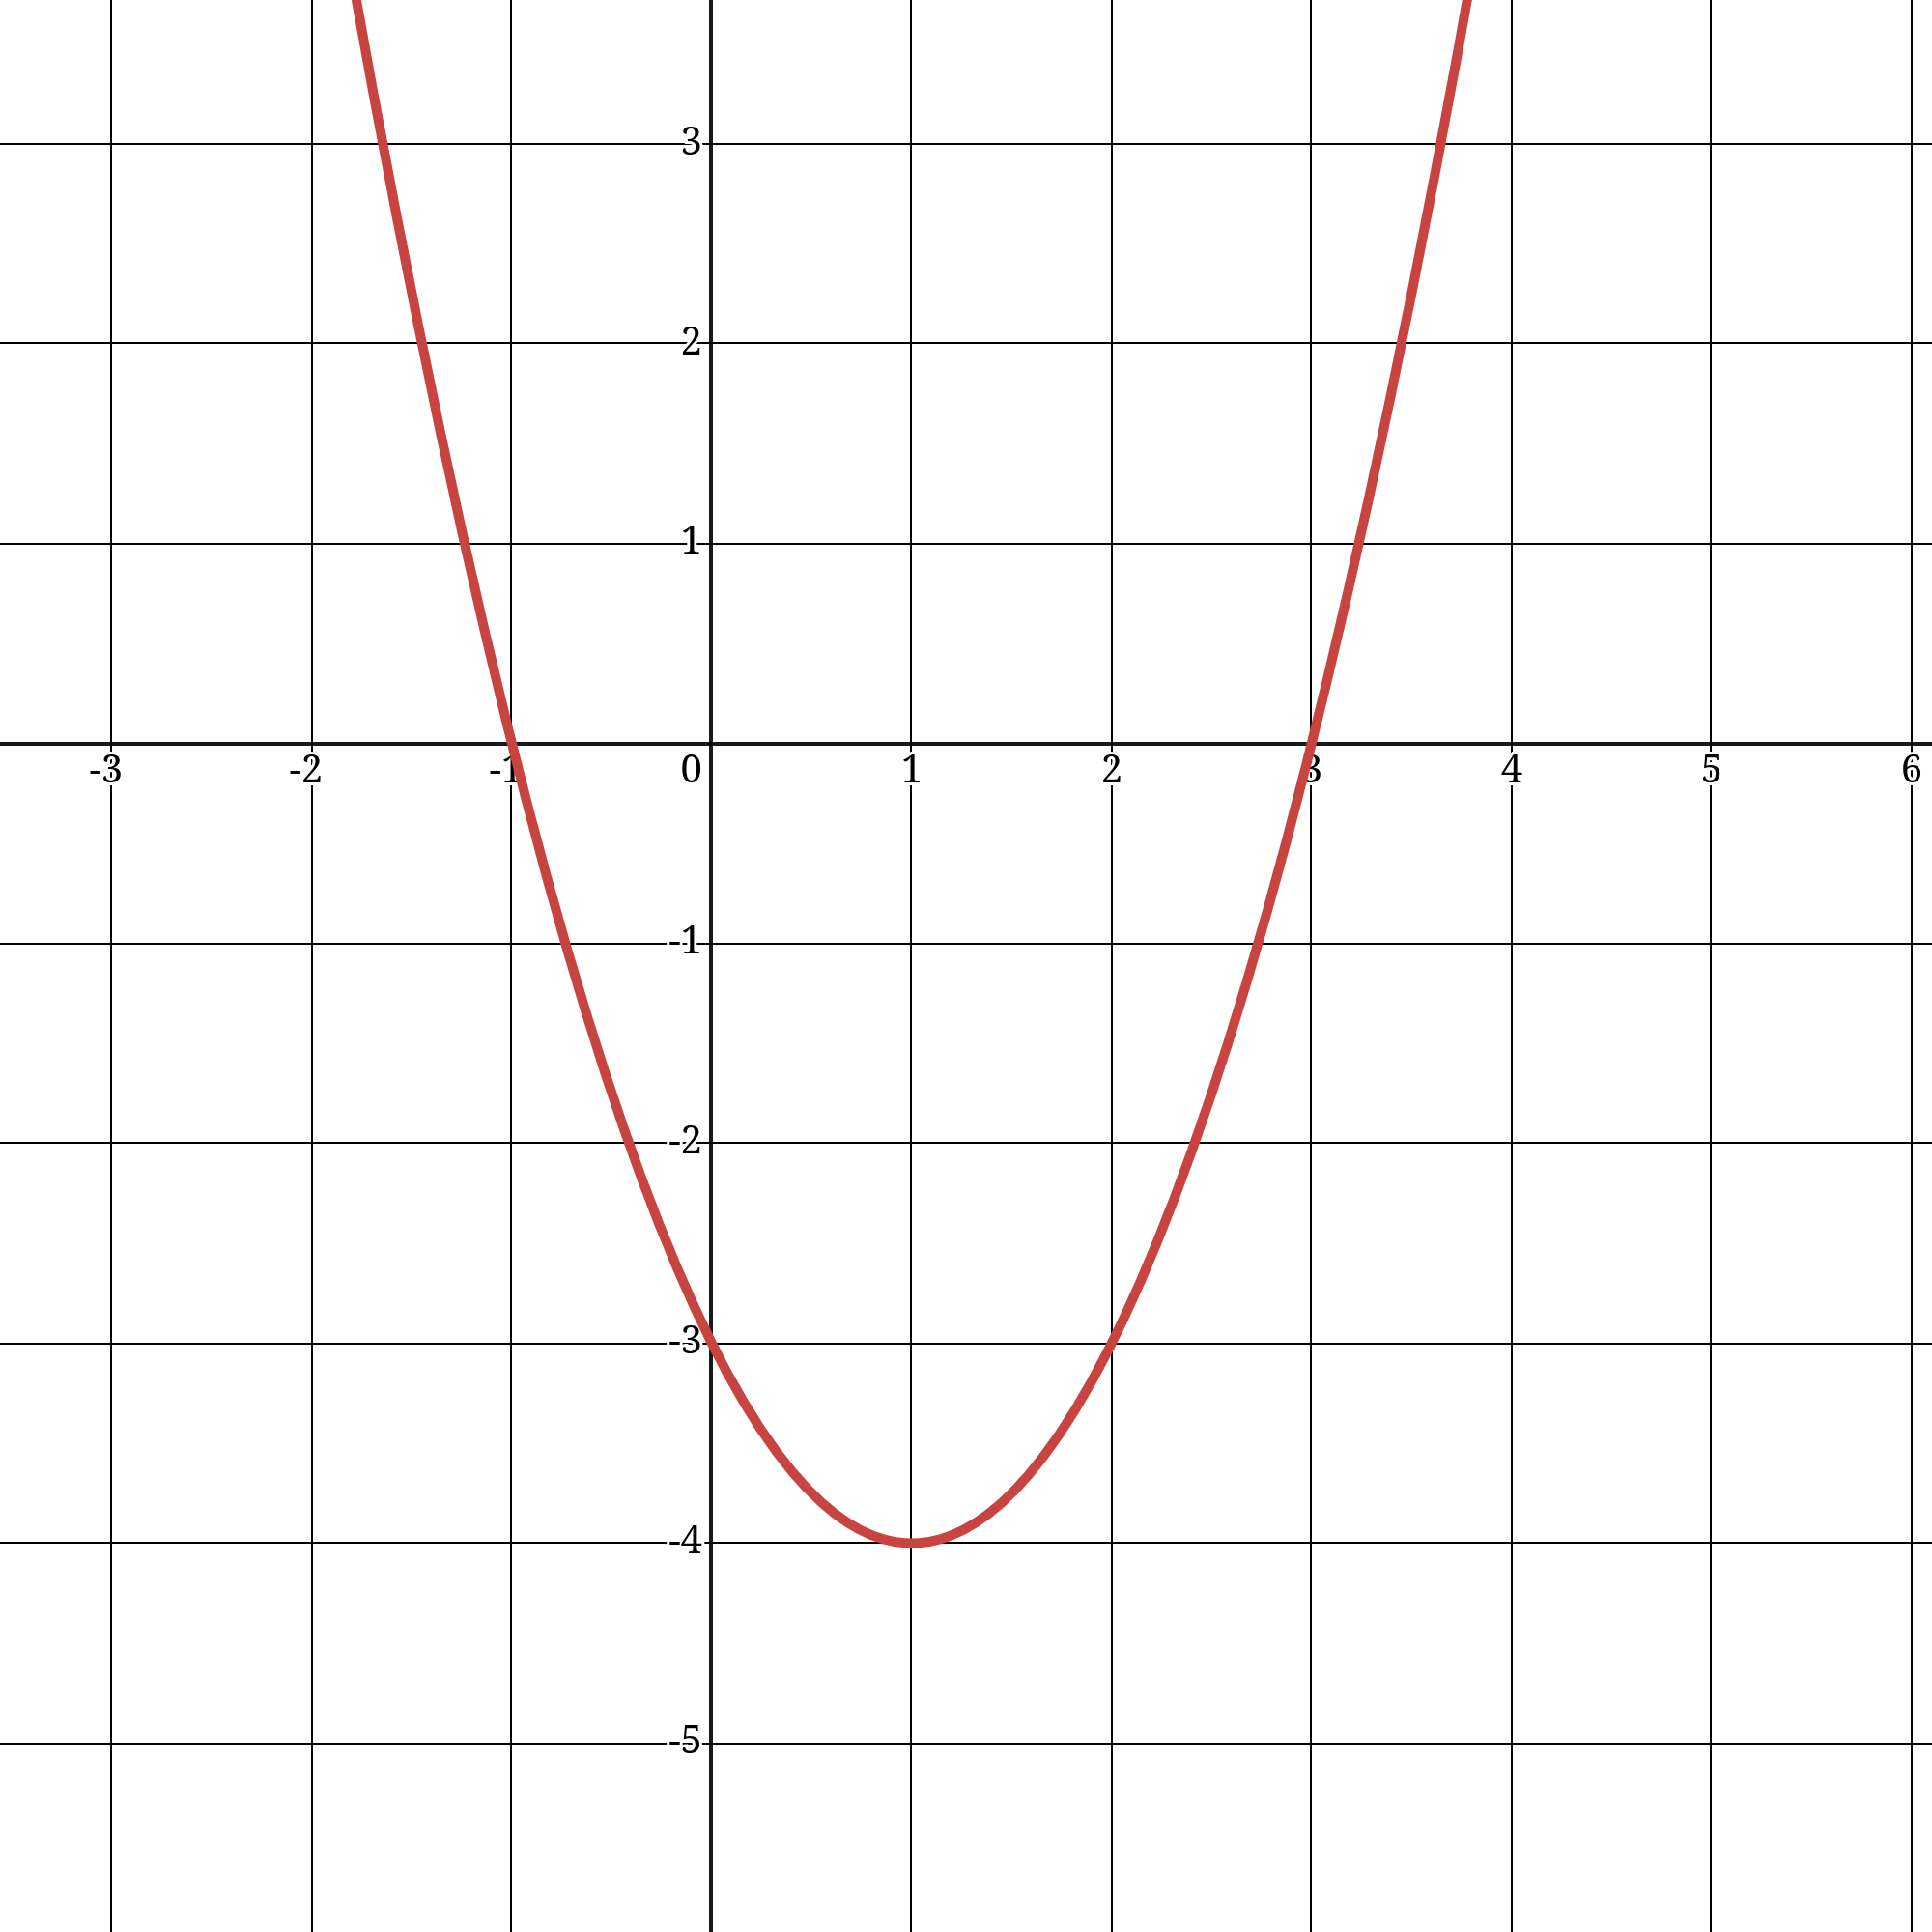
\includegraphics[scale = 0.1]{quadratic_graph}
\]

\begin{enumerate}[label = \alph*)]
    \item $f(-2) =  $ \vfill
		\item $f(0) = $ \vfill
		\item $f(1) = $ \vfill
		\item $f(2) = $ \vfill
\end{enumerate}


\question Evaluate the function
\[
f(x)=x^{2}+3
\]
for the following function values.
\begin{enumerate}[label = \alph*)]
    \item $f(-2)=$  \vfill
		\item $f(x+1)=$ \vfill
		\item $f(-x)=$ \vfill
\end{enumerate}

\newpage

\question Find the relative maximum and minimums of the following graph. . 
\[  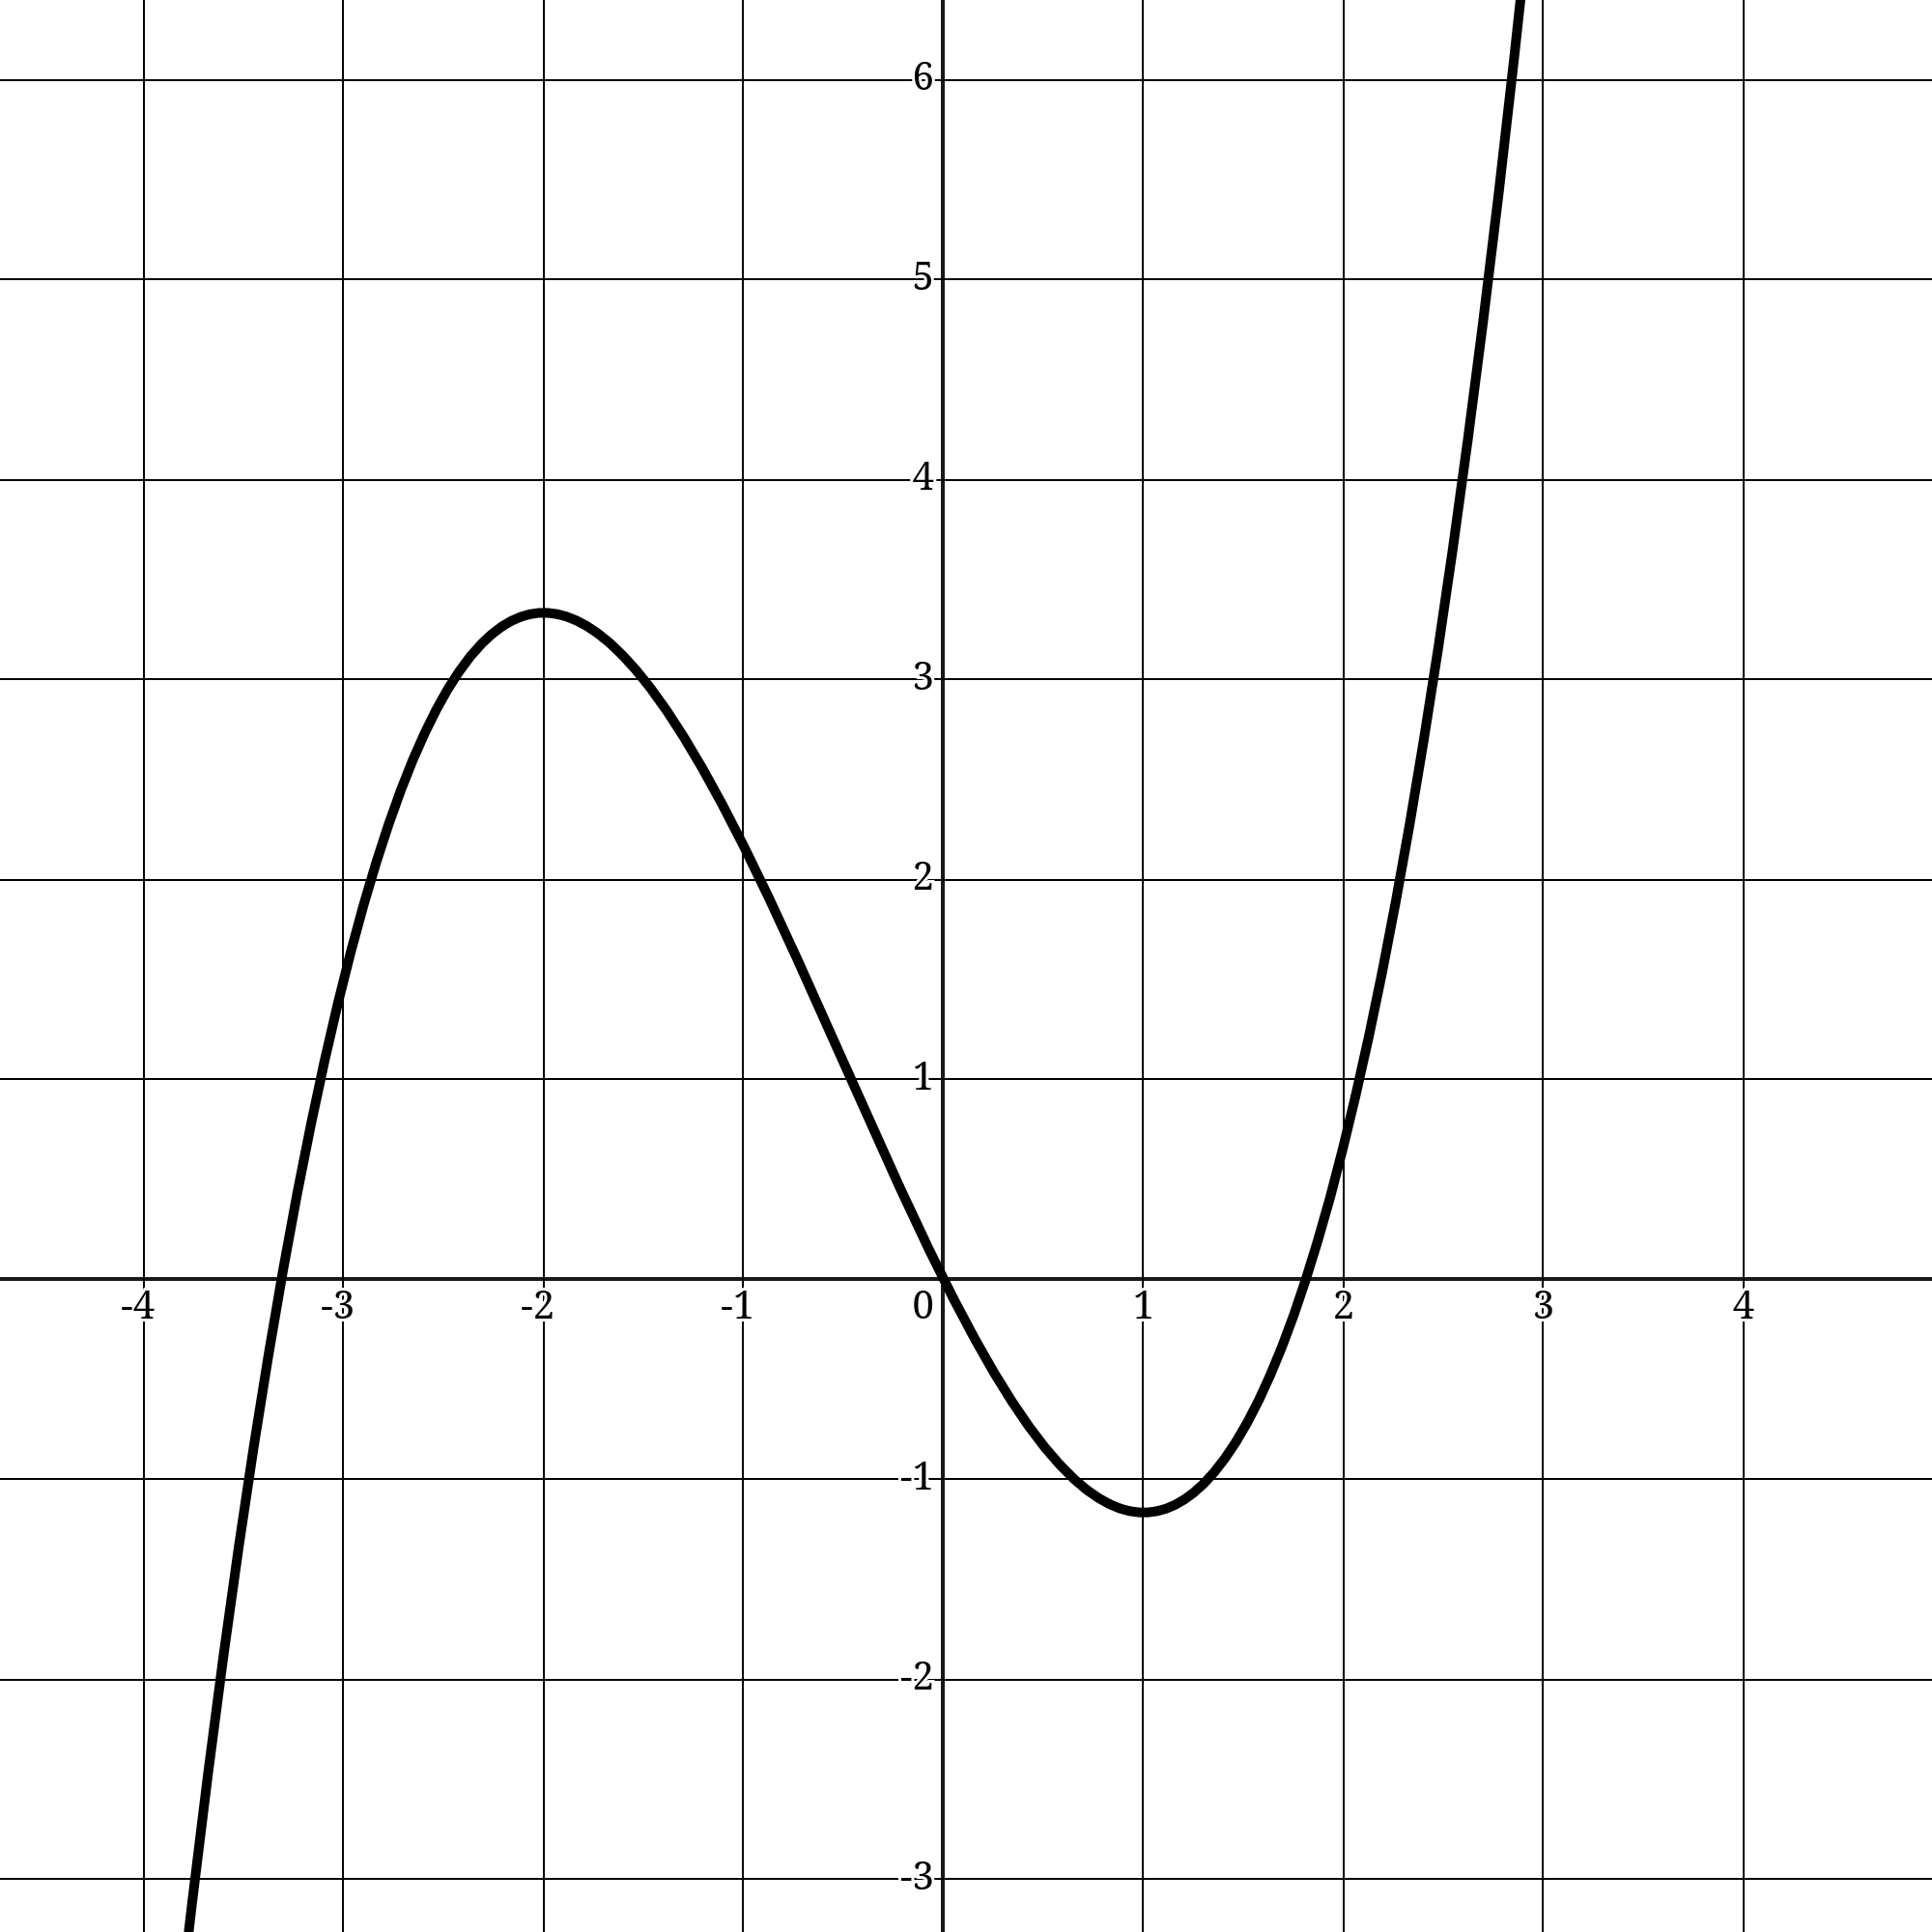
\includegraphics[scale = 0.1]{minmax}\] \vfill


\begin{comment}
\question Give an example of an even function, and verify that it is an even function. 
\end{comment}

\begin{comment}
\question Evaluate the following piecewise function at the following values
\[
	f(x) =
	\begin{cases}
   x+4 & x\leq -3 \\
	 -x+2 & x> -3 \\
	\end{cases}
\]

\begin{enumerate}[label = \alph*)]
    \item $f(-5)=$
		\item $f(-3) = $
		\item $f(-1)= $
		\item $f(0)=$
\end{enumerate}
\end{comment}

\end{questions}

\begin{theorem}[Quadratic Formula]
    Let $ax^{2}+bx +c =0$ be a quadratic equation. Then the solutions to the quadratic equation are given by 
		\[
			x = \frac{-b \pm \sqrt{b^{2} - 4ac}}{2a}
		\]
\end{theorem} \vfill

\end{document}
